\section{What is a set?}
\begin{definition}
A set is a well-defined collection of distinct objects. These objects are called \textbf{elements} or \textbf{members} of the set.

\end{definition}

\begin{remark}

In order to understand a definition as a whole, one must first break it apart into its key words, understand the meaning of those terms, then put them together to make sense of it all. Now the key words in the definition of a set are 'well-defined', 'collection', 'distinct' and 'objects'. So, roughly, a set is a bunch of objects that are \textbf{distinct} from each other and \textbf{well-defined}.
\end{remark}

\begin{example}
Consider all the planets in our solar system. The objects under consideration, planets have a standard definition %(which recently changed to exclude Pluto),
so are well-defined. No two planets are the same, so they are distinct. 

\end{example}

\begin{example}
Consider all the days in Spring when it was somewhat gloomy. Here, the objects are days that are somewhat gloomy. Since 'somewhat gloomy' is not defined precisely, this collection is not a set.

\end{example}

\paragraph{Question 1} Which of the following are sets? Explain.
\begin{enumerate}
\item All the stars in the Milky Way.
\vspace{3em}
\item All the small stars in the Milky Way.
\vspace{3em}
\item All the places that Waldo is hiding.
\vspace{3em}
\item The days in a year with exactly 20mm of rainfall.
\vspace{3em}
\item The days in 2016 in Bowling Green, Ohio with less than 20mm of rainfall.
\vspace{3em}
\item Construct your own example or counterexample of a set and explain why it is or isn't a set.
\vspace{3em}
\end{enumerate}

%\newpage
\section{How do you describe a set?}
\begin{definition}

If $A$ is a set and an object $x$ is an element of $A$, we say that $x$ \textbf{belongs to} $A$. Symbolically, we write $x \in A$. If x is not an element of A, we write $x \notin A$. 
\end{definition}

\begin{remark}
Note that sets are usually denoted by capital letters and their elements, by lower case letters.
\end{remark}

\begin{definition}
We represent a set in \textbf{tabular form} by listing out its elements, separated by commas and enclosed in brackets \{ \}.
\end{definition}

\begin{example}
If the set B consists of the primary colors red, blue and yellow, we write, B = \{red, blue, yellow\} or B = \{yellow, red, blue\}, because order doesn't matter.
\end{example}

\begin{definition}
We represent a set in \textbf{set-builder form} by stating the properties which its elements must satisfy.
\end{definition}

\begin{example}
If the set B consists of the primary colors, then we write B = \{ x : x is a primary color\}
\end{example}

\paragraph{Question 2} Answer the following:
\begin{enumerate}
\item Express the set $A=\{$x : x is a vowel$\}$ in tabular form.
\vspace{3em}
\item Express the set $B =\{A, L, G, E, B, R\}$ in set-builder form.
\vspace{3em}
\item Represent the set 'All the places that Waldo is hiding' in set-builder form, if possible.
\vspace{3em}
\item Express the set $C =\{M, I, S, P, \}$ in set-builder form..
\vspace{3em}
%\item Express the set of 'all mountains in Ohio whose peaks are above 3000 feet' in tabular form.
%\vspace{3em}
\end{enumerate}



%\newpage
\section{Types of sets}
\begin{definition}
If every element in a set A is also a member of a set B, then A is called a \textbf{subset} of B and we write $A \subset B$. If A is a subset of B, then B is a \textbf{superset} of A, or $B \supset A$.
\end{definition}

\begin{example}
If A = \{ green, yellow, red, black, dog, cat, mouse\} and B = \{dog, cat\} then  $B \subset A$
\end{example}

\begin{definition}
A set which contains no elements is called the \textbf{null set} or \textbf{empty set} and we denote it by the symbol $\emptyset$.
\end{definition}

\begin{remark}
From the two definitions above we can conclude that the null set is a subset of every set because the null set contains no elements, hence all members of the null set is are members of every set!
\end{remark}

\begin{definition}
A set which contains only a single element is called a \textbf{singleton set}
\end{definition}

\begin{example}
The set of tallest mountains on earth is a singleton set, since there is a unique tallest mountain on earth, Mt. Everest.
\end{example}


\paragraph{Question 3-A}
For the following questions, identify the sets in the context of the definitions above.
\begin{enumerate}
    
    \item If $A$ is the set of all cars manufactured by a Japanese car company and $B$ is the set of all Toyota sedans, then what is the relationship between $A$ and $B$?
    \vspace{3em}
    
    \item If Jill has classes on Mondays, Wednesdays and Fridays and has work on Saturdays and Wednesdays, then what type of set is the set of days on which Jill has both work and classes?
    \vspace{3em}
    
    \item Bob sends Alice a message every 5 hours, on the hour, but Alice can only receive messages every three hours, on the hour. If a message is not received when it is sent, it is lost. Assume that both Alice and Bob start sending and receiving messages at the same time. If $R$ is the set of messages that Alice has received from Bob and $S$ is the set of messages that Bob has sent out, what is the relation between the sets $R$ and $S$? You may assume that one message counts for one element in the set.
    \vspace{5em}

    
\end{enumerate}






%\newpage
\begin{definition}
If all the sets under investigation are subsets of a fixed set, this set is called the \textbf{universal set} or \textbf{universe of discourse} and denoted by \textbf{U}.
\end{definition}

\begin{example}
If we were surveying the number of people of each nationality, the universal set would consist of all the people on earth.
\end{example}

\begin{example}
If we were studying the stars in the Milky Way, the universal set consists of all the stars in the universe.
\end{example}

\begin{definition}
If two sets A and B have no elements in common, we say that they are \textbf{disjoint} sets.
\end{definition}

\begin{example}
The set consisting of all World War II veterans and the set of all millennials are disjoint sets. 
\end{example}

\paragraph{Question 3-B}
For the following questions, identify the sets in the context of the definitions above, where applicable.
\begin{enumerate}
    
    \item In the question about Alice in Bob in 3-A, what type of set is $S$? Explain.
    \vspace{5em}
    
    \item Is it possible for the Universal set to be empty? Explain why or why not.
    \vspace{5em}
    
    \item If two sets $A$ and $B$ are subsets of a given universal set, $U$, is it possible that $A = U$ or $B = U$? Explain why or why not.
    \vspace{5em}
    
    \item Is it possible for the universal set to be disjoint from any of its subsets? Explain why or why not.
    \vspace{5em}

    
    
\end{enumerate}







%\begin{definition}
%When the objects of a set are set themselves, we call them a \textbf{family of sets} or a \textbf{class of sets}
%\end{definition}

%\begin{definition}
%the \textbf{power set} of any set S is the set of all subsets of S, including the empty set and S itself. The power set of a set S is usually denoted by \textbf{P(S)},
%\end{definition}








%\newpage
\section{Comparing sets}
\begin{definition}
Set A is equal to set B if they both have the same elements. We write this as $A=B$.
\end{definition}

\begin{example}
The set consisting of all colors of a rainbow and the component colors of white light observer through a dispersion prism are equal sets.
\end{example}

\begin{definition}
The number of elements in a set A is the \textbf{cardinality} of the set and is denoted by $\left| A\right|$ 
\end{definition}

\begin{definition}
If two sets A and B have the same cardinality, we say they are \textbf{equivalent} and write $A \sim B$
\end{definition}

\begin{example}
The B = \{Tesla, Frisker\} and C = \{Ford, Toyota\} are not comparable, nor are they equal, but they are equivalent, since $\left| B\right|$ = $\left| C\right|$.
\end{example}

\begin{definition}
Two sets A and B are \textbf{comparable} if $A \subset B$ or $B \subset A$. If this is not the case, then they are said to be \textbf{not comparable}.
\end{definition}

\begin{example}
The sets A = \{General Motors, Toyota, Ford, Renault\} and B = \{Tesla, Frisker\} are not comparable, where as C = \{Ford, Toyota\} and A are comparable, since $C \subsetneq A$.
\end{example}

\begin{definition}
If B is a subset of A and B is not equal to A then we say that B is a \textbf{proper subset} of $A$ and write $B$ $\subsetneq$ $A$.
\end{definition}

\paragraph{Question 4}
For the following questions, compare the sets in the context of the definitions above. If they are not comparable, explain why.
\begin{enumerate}
    
    \item The set of humans that have been to more than one planet and the set of humans that have been to Pluto.
    \vspace{5em}
    
    \item The set $A = \{ \divideontimes, \boxtimes, \blacktriangleleft, \boxplus \} $ and the set $B = \{ \boxplus, \blacktriangleleft, \divideontimes, \boxtimes \} $
    \vspace{5em}
    
    \item The set consisting of the members of the Green Bay Packers on the in play during a game and the set consisting of the members of the Manchester United soccer team in play during a game.
    \vspace{5em}
    
    \item The set consisting of all employees of the Department of Justice and the set consisting of all federal employees.
    \vspace{5em}
    
    \item Is it possible for two set to be comparable but not equivalent? Explain why or why not.
    \vspace{5em}
    
    
\end{enumerate}




%\newpage
\section{Set Operations I}
\begin{definition}
The \textbf{union} of sets A and B is the set of all elements which belong to A or to B or to both. We denote this by $A \cup B$.
\end{definition}

\begin{definition}
The \textbf{intersection} of sets A and B is the set of elements which belong to both A and B. We denote this by $A \cap B$.
\end{definition}



\paragraph{Question 5} Answer the following, expressing the answers as sets where possible.
\begin{enumerate}
\item If $X=\{Tom, Dick, Harry\}$, $Y=\{Tom, Marc, Eric\}$, $Z=\{Marc, Eric, Edward\}$ Find:
\begin{enumerate}
\item $X \cup Y$
\vspace{3em}
\item $Y \cup Z$
\vspace{3em}
\item $X \cup Y \cup Z$
\vspace{3em}
\item $X \cap Y \cap Z$
\vspace{3em}
\end{enumerate}
\item Is it true that $A \cup B=B \cup A$? Explain. 
\vspace{5em}
\item If $A\subset B$ then what is $A \cup B$?
\vspace{5em}
\item Is $A \cap B$ a subset of $A$? Is $A \cap B$ a subset of $B$? Explain.
\vspace{5em}
\item What is $A \cap A$? What about $A \cup A$?
\vspace{5em}
\item What is $\emptyset \cap A$? Does it depend on the set $A$? Explain why or why not.
\vspace{5em}
\item What is $\emptyset \cup A$? Does it depend on the set $A$? Explain why or why not. 
\vspace{5em}
\item If $A \cup B=\emptyset$, what can we say anything about $A$ or $B$? Is there something special about them? Explain.
\vspace{5em}
\item If $A$ and $B$ are disjoint, what can we say about $A \cap B$?
\vspace{5em}
\item If $A\subset B$ and $B$ and $C$are disjoint, then what about $A$ and $C$?
\vspace{5em}
\item If $U$ denotes the universal set, is it true that $U \cap A=A \cap \emptyset$? Explain.
\vspace{5em}

\end{enumerate}



%\newpage
\section{Venn Diagrams}
\begin{definition}
A Venn diagram (also called \textbf{primary diagram}, \textbf{set diagram} or \textbf{logic diagram}) is a diagram that shows all possible logical relations between a finite collection of different sets. These diagrams depict elements as points in the plane, and sets as regions inside closed curves. A Venn diagram consists of multiple overlapping closed curves, usually circles, each representing a set.
\end{definition}

\begin{remark}
This definition might seem complicated, but for our purposes we will think of Venn diagrams as circles that represent sets. The following examples will help make this clear.
\end{remark}

\begin{example}
In general, If we want to represent a single set using a Venn diagram, we draw a single circle (representing the set) inside a rectangle (representing the universal set).

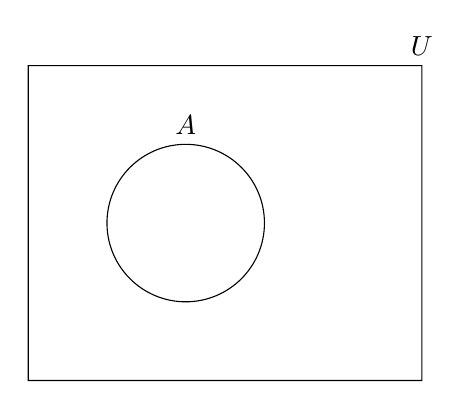
\begin{tikzpicture}[fill=gray]

% outline
\draw (0,0) circle (1) (0,1)  node [text=black,above] {$A$}
      %(1,0) circle (1) (1,1)  node [text=black,above] {$B$}
      (-2,-2) rectangle (3,2) node [text=black,above] {$U$};
\end{tikzpicture}
\end{example}


\begin{remark}
We usually write the label for a given set above the circle that represents it.
\end{remark}


\begin{example}
The representation in the above example can be extended to any finite number of sets. If want to represent two sets, A and B, we can represent them as below:

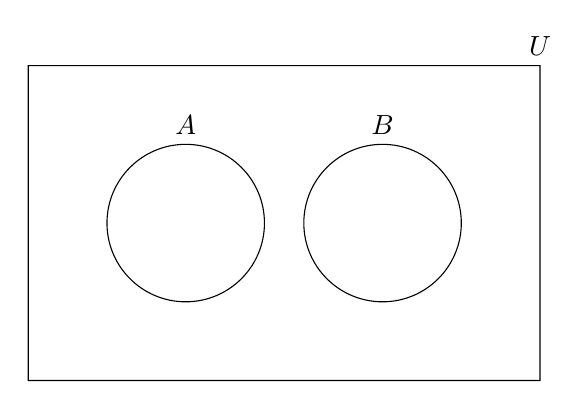
\begin{tikzpicture}[fill=gray]

% outline
\draw (0,0) circle (1) (0,1)  node [text=black,above] {$A$}
      (2.5,0) circle (1) (2.5,1)  node [text=black,above] {$B$}
      %(5,0) circle (1) (5,1)  node [text=black,above] {$C$}
      (-2,-2) rectangle (4.5,2) node [text=black,above] {$U$};
\end{tikzpicture}

\end{example}




%\newpage
\begin{remark}
The power of Venn diagrams is that they make it easy to understand set operations. Let's look at a few examples.
\end{remark}

\begin{example}
If B is a subset of A, we can represent this as below:

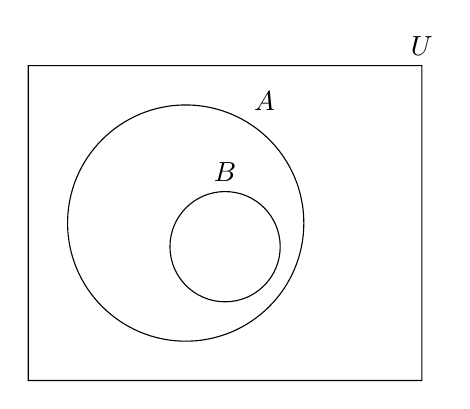
\begin{tikzpicture}[fill=gray]

% outline
\draw (0,0) circle (1.5) (1,1.3)  node [text=black,above] {$A$}
      (0.5,-0.3) circle (0.7) (0.5,0.4)  node [text=black,above] {$B$}
      (-2,-2) rectangle (3,2) node [text=black,above] {$U$};
\end{tikzpicture}

\end{example}

\newpage
\begin{example}
For two sets A and B which may or may not be disjoint, we represent $A \cap B$ as below:


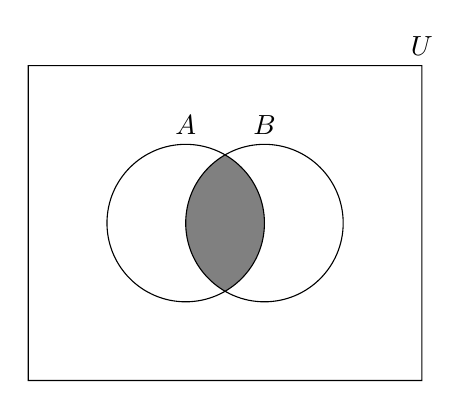
\begin{tikzpicture}[fill=gray]

\scope % A \cap B
\clip (0,0) circle (1);
\fill (1,0) circle (1);
\endscope

% outline
\draw (0,0) circle (1) (0,1)  node [text=black,above] {$A$}
      (1,0) circle (1) (1,1)  node [text=black,above] {$B$}
      (-2,-2) rectangle (3,2) node [text=black,above] {$U$};
\end{tikzpicture}

\end{example}

\begin{example}
If we know that A and B, are not disjoint, we indicate this by a dot inside the region of their overlap.


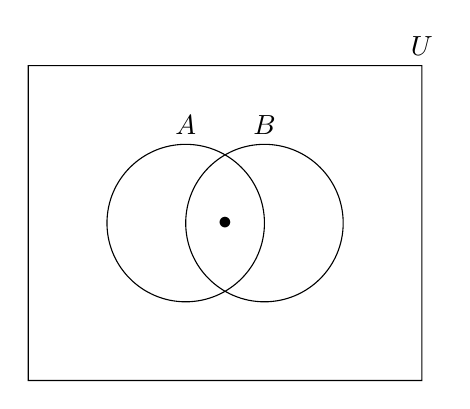
\begin{tikzpicture}[fill=gray]

\scope % A \cap B
\clip (0,0) circle (1);
%\fill (1,0) circle (1);
\endscope

% outline
\draw (0,0) circle (1) (0,1)  node [text=black,above] {$A$}
      (1,0) circle (1) (1,1)  node [text=black,above] {$B$}
      (0.5,-0.2) node [text=black,above] {$\bullet$}
      (-2,-2) rectangle (3,2) node [text=black,above] {$U$};
\end{tikzpicture}

\end{example}



\begin{example}
If B is a proper subset of A, we can represent this with a dot outside B, but within A.

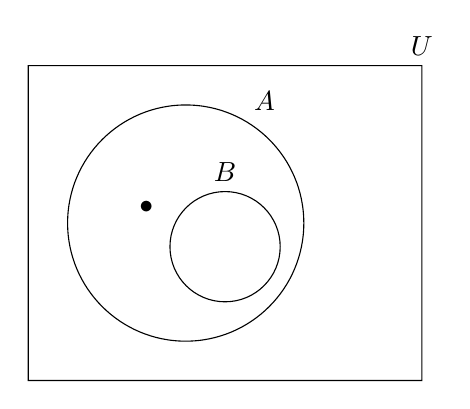
\begin{tikzpicture}[fill=gray]

% outline
\draw (0,0) circle (1.5) (1,1.3)  node [text=black,above] {$A$}
      (0.5,-0.3) circle (0.7) (0.5,0.4)  node [text=black,above] {$B$}
      (-0.5,0) node [text=black,above] {$\bullet$}
      (-2,-2) rectangle (3,2) node [text=black,above] {$U$};
\end{tikzpicture}

\end{example}



\begin{example}
For two sets A and B, we represent $A \cup B$ as below:

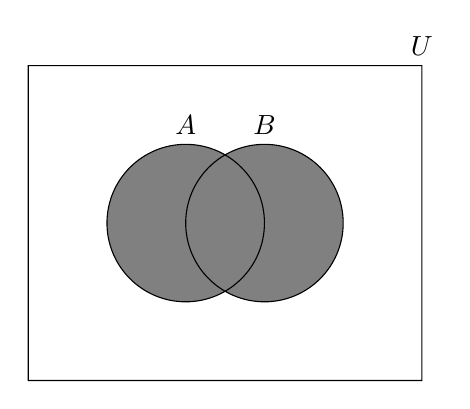
\begin{tikzpicture}[fill=gray]

\scope % A \cap B
\fill (1,0) circle (1);
\fill (0,0) circle (1);
\endscope

% outline
\draw (0,0) circle (1) (0,1)  node [text=black,above] {$A$}
      (1,0) circle (1) (1,1)  node [text=black,above] {$B$}
      (-2,-2) rectangle (3,2) node [text=black,above] {$U$};
\end{tikzpicture}


\end{example}
\newpage
\begin{example}
For three sets A, B and C, we represent $A \cap B \cap C$ as below:

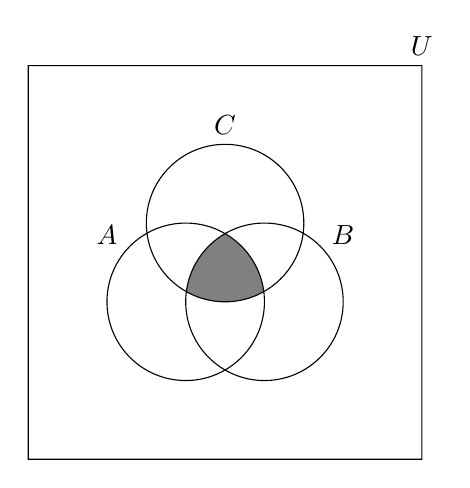
\begin{tikzpicture}[fill=gray]

\scope % A \cap B
\clip (0,0) circle (1);
\clip (0.5,1) circle (1);
\fill (1,0) circle (1);
\endscope

% outline
\draw (0,0) circle (1) (-1,0.6)  node [text=black,above] {$A$}
      (1,0) circle (1) (2,0.6)  node [text=black,above] {$B$}
      (0.5,1) circle (1) (0.5,2)  node [text=black,above] {$C$}
      (-2,-2) rectangle (3,3) node [text=black,above] {$U$};
\end{tikzpicture}
\end{example}







%\newpage
\paragraph{Question 6}
For the following questions, represent your answers as Venn diagrams, where possible. If a Venn diagram is not possible, explain why.
\begin{enumerate}
    
    \item $A \cup B$, given that $A$ and $B$ are disjoint.
    \vspace{8em}
    
    \item $(A\cap B)\cup C$, given that $C$ is disjoint from $B$.
    \vspace{8em}
    
    \item $A\cap B \cap C$, given that each of $A$, $B$ and $C$ is disjoint from the other two.
    \vspace{8em}
    
    \item If $A$ and $B$ are not disjoint and $C \subsetneq B$ but is disjoint from $A$, how would you represent this? 
    \vspace{8em}
    
    \item If $A \cap B \subsetneq C$, but $C \subsetneq A \cup B$, how would you represent this?
    \vspace{8em}
    
    
\end{enumerate}









%\newpage
\section{Set Operations II}

\begin{definition}
The \textbf{complement} of a set A is the set of elements that do not belong to A. Therefore, it is the difference of the universal set U and A. We denote the complement of A as $A^c$ or $A'$. Visually, we represent this as:

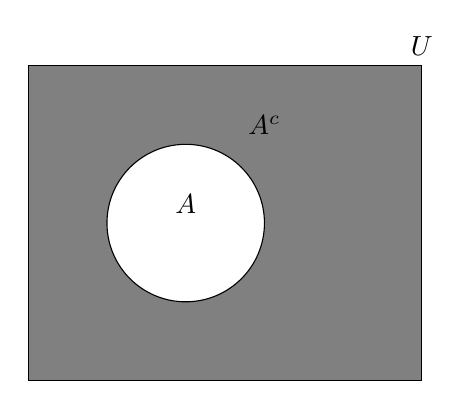
\begin{tikzpicture}[fill=gray]
\scope % A^c
    \filldraw   (-2,-2) rectangle (3,2) node [text=black,above] {$U$};
    \fill[white] (0,0) circle (1);
\endscope
% outline
\draw (0,0) circle (1) (0,0)  node [text=black,above] {$A$}
      (1,1)  node [text=black,above] {$A^c$};
\end{tikzpicture}

\end{definition}


\begin{definition}  
The \textbf{difference} of sets A and B is the set of elements which belong to A but not to B. We denote this as $A-B$ or $A \setminus B$. Visually, we represent this as:

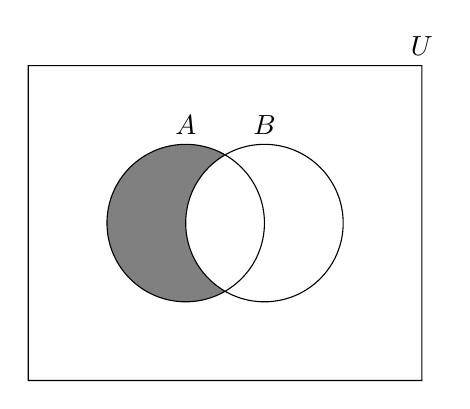
\begin{tikzpicture}[fill=gray]
% left hand
\scope
\clip (-2,-2) rectangle (2,2)
      (1,0) circle (1);
\fill (0,0) circle (1);
\endscope
% right hand
%\scope
%\clip (-2,-2) rectangle (2,2)
      %(0,0) circle (1);
%\fill (1,0) circle (1);
%\endscope
% outline
\draw (0,0) circle (1) (0,1)  node [text=black,above] {$A$}
      (1,0) circle (1) (1,1)  node [text=black,above] {$B$}
      (-2,-2) rectangle (3,2) node [text=black,above] {$U$};
\end{tikzpicture}

%TODO: explain difference of sets as relative complement

\end{definition}

%TODO: add a remark explaining the concept of relative complement

%\begin{definition}
%The \textbf{Cartesian product} of two sets A and B, denoted by A $\times$ B is the set of all ordered pairs $(a,b)$ where a $\in$ A and b $\in$ B. It can be specified using set-builder notation, i.e. $A \times B=\{(a,b) : a\in A$ and  $b\in B\}$.
%\end{definition}






\paragraph{Question 7}
For the following questions, represent your answers as Venn diagrams, where possible.
\begin{enumerate}
    
    \item $(A \cap B)^c$, given that $A$ and $B$ are not disjoint.
    \vspace{8em}
    
    \item $(A^c \cup B^c)$, given that $A$ and $B$ are not disjoint.
    \vspace{8em}
    
    \item $A^c \setminus B$.
    \vspace{8em}
    
    \item $A \setminus B$, given that $B \subsetneq A$. 
    \vspace{8em}
    
    %\item Tammy is ordering a pizza and has the choice of three crusts: pan, regular or hand-tossed. She can choose Alfredo, Marinara or Pesto sauce and can add either peppers, mushrooms or spinach  as a topping and has to choose between mozzarella and feta cheese. Let the set of available crusts be C, sauces be S, toppings be T and cheeses be H. If Tammy doesn't like mushrooms and doesn't like feta cheese, how would you use set builder notation to represent the different pizzas she could order? 
    \vspace{5em}
    
    
\end{enumerate}


